\documentclass[12pt,letterpaper, onecolumn]{exam}
\usepackage{amsmath}
\usepackage{amssymb}
\usepackage{graphicx}
\usepackage[lmargin=71pt, tmargin=1.2in]{geometry}  %For centering solution box
\usepackage{listings}
\lstset{
    basicstyle=\ttfamily\footnotesize,  % font size and style
    breaklines=true,                    % wrap long lines
    frame=single,                       % add a frame around the code
    xleftmargin=10pt,                   % left margin
    xrightmargin=10pt,                  % right margin
    aboveskip=10pt,                     % space before the listing
    belowskip=10pt,                     % space after the listing
}

% \chead{\hline} % Un-comment to draw line below header
\thispagestyle{empty}   %For removing header/footer from page 1

\begin{document}

\begingroup  
    \centering
    \LARGE STATS 212\\
    \LARGE Homework#3 \\
    \large \today\\[0.5em]
    \large Samuel Molero\par
    \large samueljosemolero@tamu.edu\par
    \large Section: 501\par
\endgroup
\rule{\textwidth}{0.4pt}
\pointsdroppedatright   %Self-explanatory
\printanswers
\renewcommand{\solutiontitle}{\noindent\textbf{Ans:}\enspace}   %Replace "Ans:" with starting keyword in solution box

\begin{questions}

    \question Q1?
    \begin{solution}
        \begin{parts}
        \part 
        \begin{verbatim}
            df <- read.csv("Baseball-Salary-Data.csv")
            head(df)
            m1 <- lm(salary ~ . - player, data = df)
            summary(m1)
        \end{verbatim}
        Running the above code output the following results:\\
        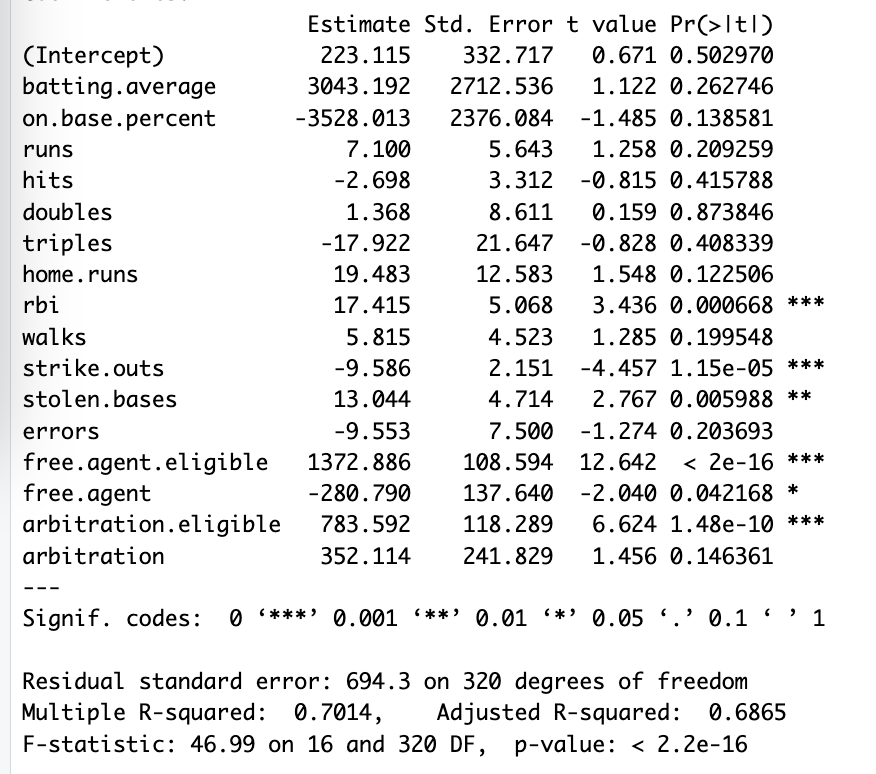
\includegraphics[width=0.7\textwidth]{Homeworks/HW3A.png}
        \part The R square of 0.7014, which translates to 70.14\%\
        \part The coefficient for the predictor is -2.698 which predicts a decrease in salaries holding all the other variables constant.This could be due to the variation in salary data is explained by other variables such as home run and stolen bases.
        \part  Given that the P-value is 2.2e-16, which is smaller than 0.05 thus rejecting the null. This means that the model has good utility, and is a helpful indicative at predicting salary data.
        \part Give that the F statistic is 0.619 and that is bigger than the give alpha, the second model does not have a significant improvement at predicting the Salary compared to the first model. This result is surprising became you would assume that having less predictors would make the prediction of salary worse given that there is less information.
        \part This value will be the R-squared which is 0.6981 about 69.81\%\
        \part 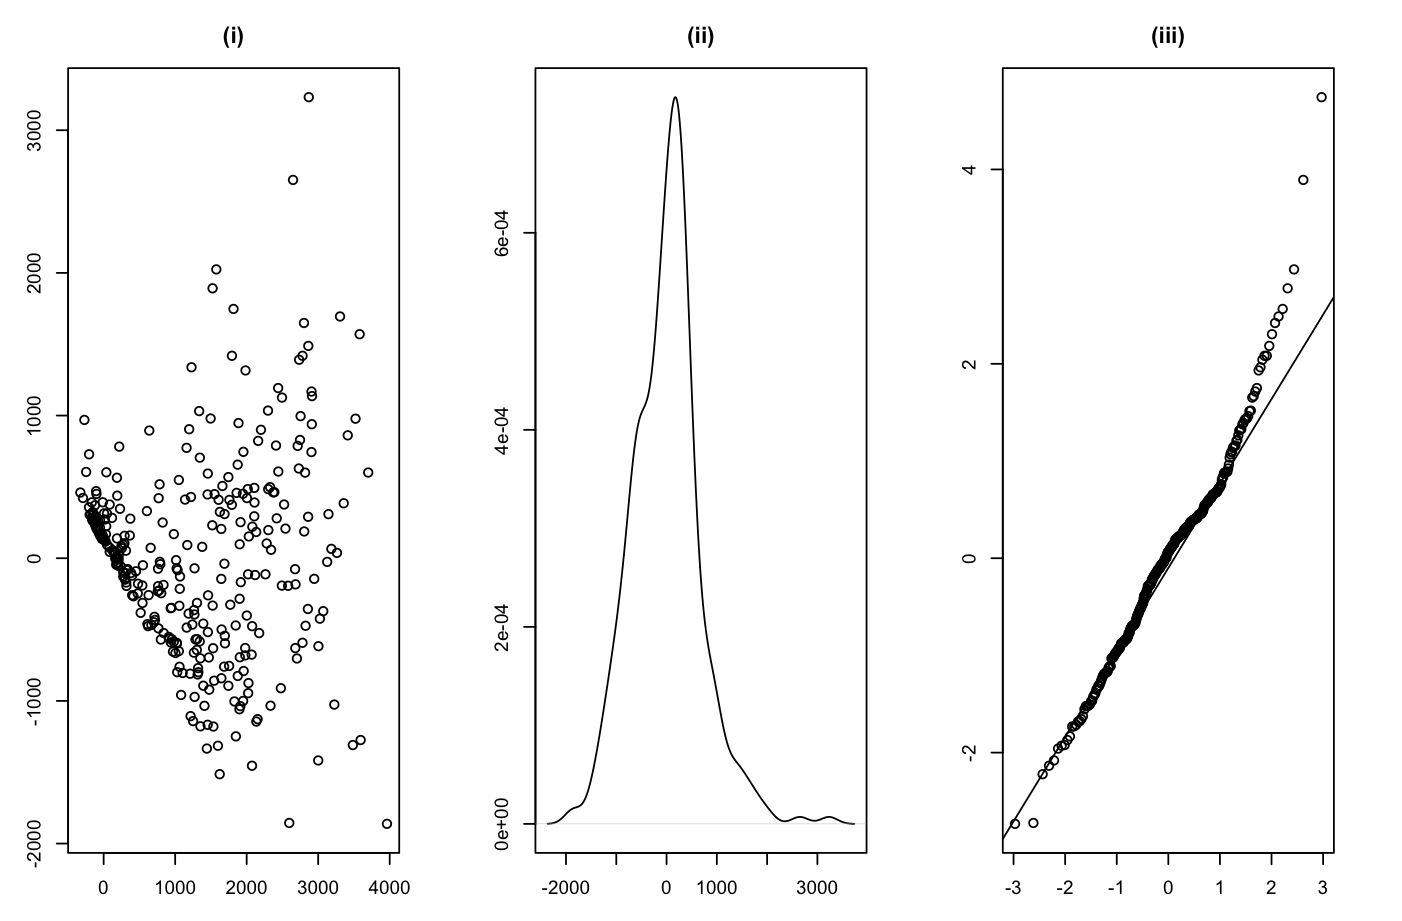
\includegraphics[width=0.96\textwidth]{Homeworks/Plots1232.png}\\
            (i) The is no clear pattern, but the spread of residuals increases in proportion to fitted values, indicating no constant variance. Additionally, non-linearity exits which demonstrate that a linear model may not be the best fit.\\
            (ii) The distribution is highly skewed, indicating for no normality assumption. \\
            (iii) The points mostly follow a straight line in the middle, but deviate at extremes demonstrating a non-normality.\\
        \part 
        \begin{lstlisting}
    source("AIC-Leaps.R")
    df <- read.csv("Baseball-Salary-Data.csv")
    df <- df[, -18]
    
    library(leaps)
    leaps_ic <- leaps.AIC(df[,2:17], df[, 1])
        # includes all predictors             includes the response variable
    leaps_output <- leaps(df[, 2:17], y = df[, 1], nbest = 1) # perform AIC\BIC calc
    
    var_names <- colnames(df[, 2:17]) # get predictors name
    best_model_index <- which.min(leaps_output$Cp) # Get selected variables
    var_mask <- leaps_output$which[best_model_index, ] 
    model_vars <- var_names[var_mask] # extract the best predictor names
    model_vars
    \end{lstlisting}
    By the code above,the best predictors are "home.runs", "rbi","walks",\\
    "strike.outs",\\
   "stolen.bases","free.agent.eligible","free.agent","arbitration.eligible",\\
    and "arbitration" \\   
        
    The rationale for selecting these predictors was based on the combination of player performance metrics and contractual factors that ultimately influence the salary. The leaps() function alongside Mallows CP helps identify the best subset, by comparing the models' goodness of fit and complexity. A lower CP will indicate that the model is both accurate and not complex, which is why the models with the lowest CP were selected as the best subset, to ensure that the salary variations are explained without unnecessary predictors, and thus show  the strongest statistical relation with salary.\\

        \part
        \begin{verbatim}
            
        \end{verbatim}
        \end{parts}
        
            
    \end{solution}
    
    \question Q2?
    \begin{solution}
        \begin{parts}
            \part 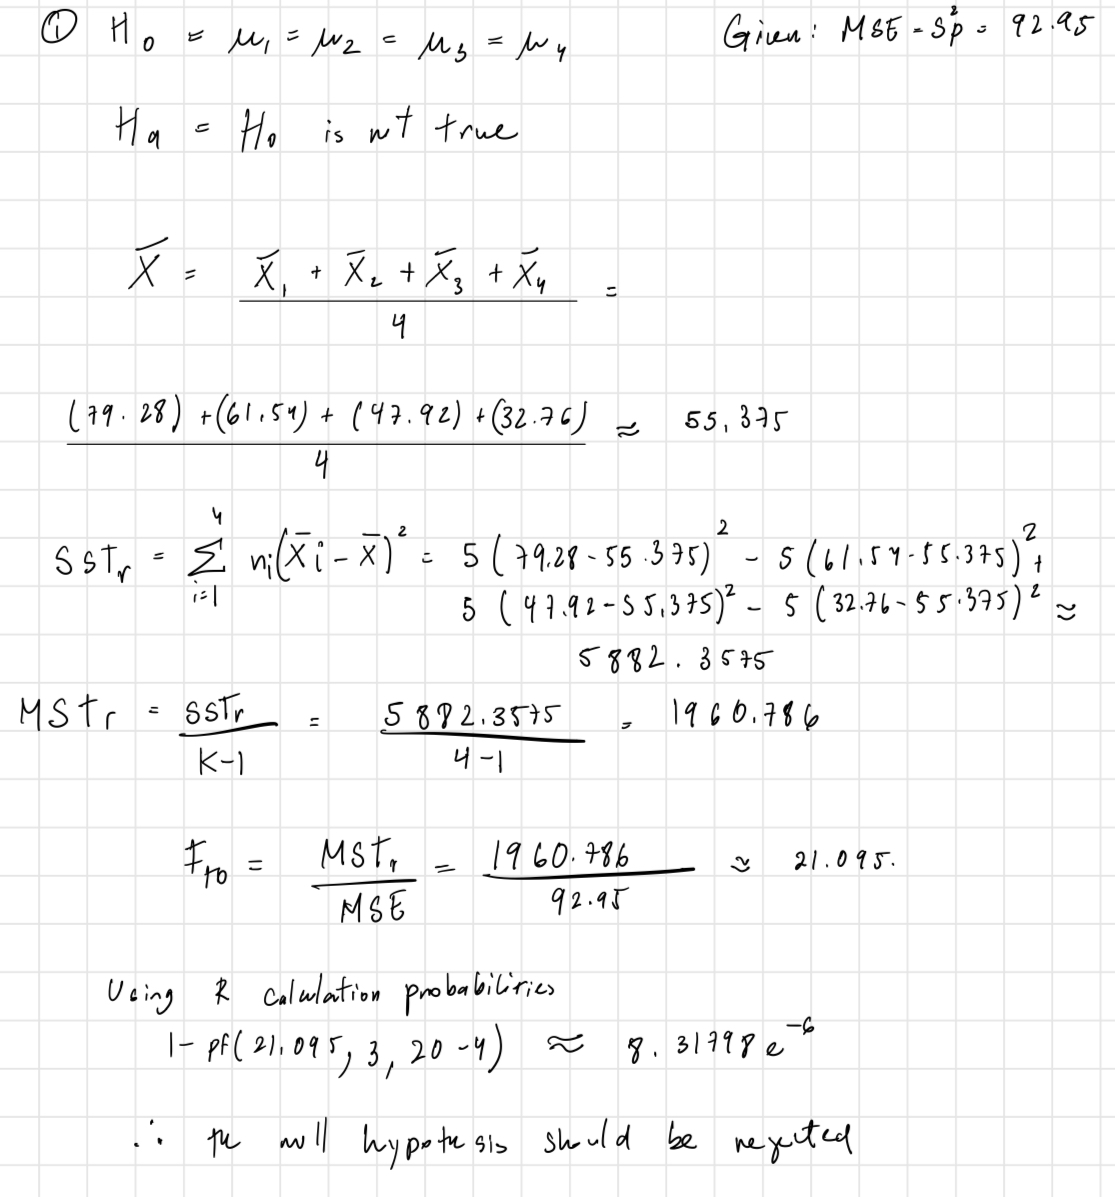
\includegraphics[width=0.7\textwidth]{Homeworks/partAHW3.jpg}
            \part
            \begin{verbatim} 
    dta2 <- read.table("SleepRem.txt", header = TRUE, sep = "")
    attach(dta2)
    fit <- aov(values ~ as.factor(ind), data = dta2)
    anova(fit)
    \end{verbatim}
    Using the above code snippet we get the following result:
    \begin{verbatim}
Response: values
        Df  Sum Sq  Mean Sq  F value  Pr(>F)    
find     3  5881.7 1960.58  21.093 8.322e-06 
Residuals 16 1487.1   92.95                      
    \end{verbatim}
    Given that is confirmed that the p-value is $8.322e-06$ the null hypothesis should be rejected.
    \part 
    \begin{verbatim}
      #To test variance
      anova(aov(resid(aov(values ~ ind))**2 ~ ind))
    \end{verbatim}
    Given that the p-value is 0.621. This suggests that the assumption of equal
    variance is approximately valid.
    \begin{verbatim}
    #to test stability
    shapiro.test(resid(aov(values ~ ind)))
    \end{verbatim}
     p-value = 0.1285 suggests that the normality assumption
    approximately holds.
    \end{parts}
    \begin{verbatim}
        fit = aov(values ~ find)
        boxplot(resid(fit))
        plot(fit, which=2)
        \end{verbatim}
       The Code snippets creates the following graphs:\\
    \center
    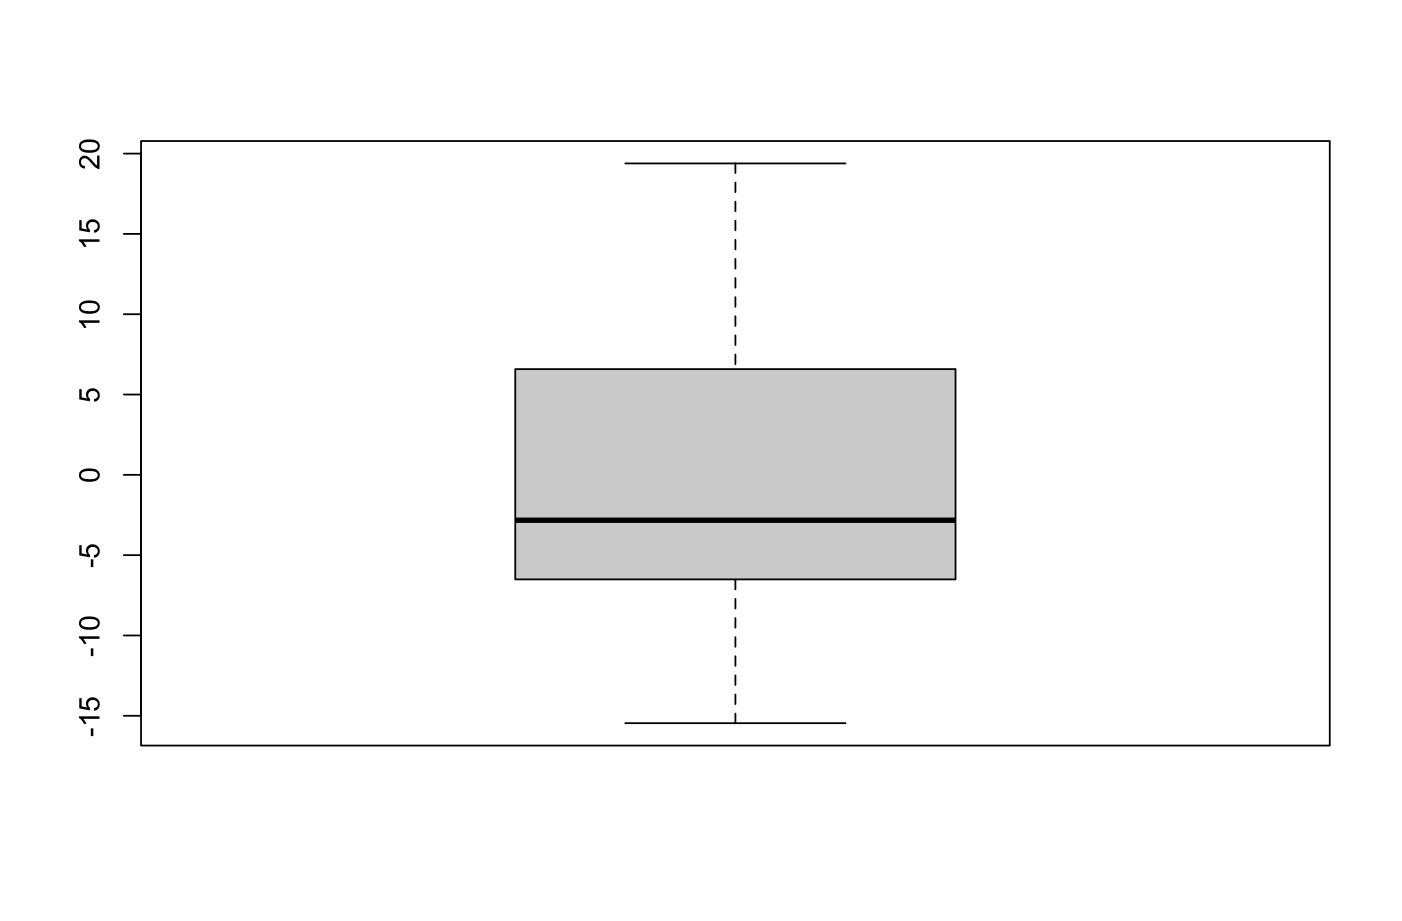
\includegraphics[width=0.7\textwidth]{Homeworks/Graph1HW3.png}\\
    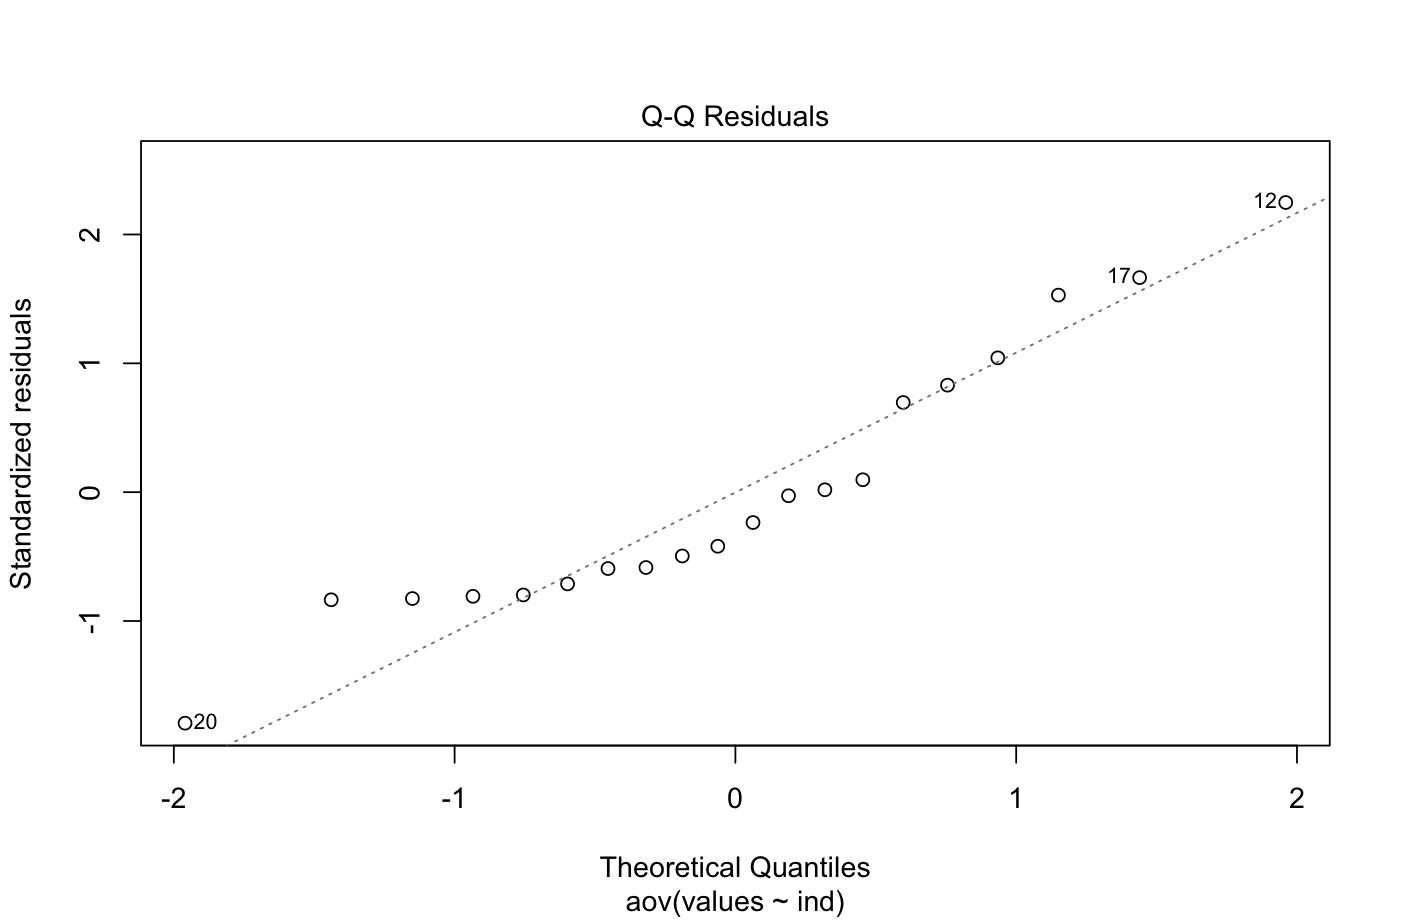
\includegraphics[width=0.7\textwidth]{Homeworks/Graph2HW3.png}\\
    plots also suggest that the normality assumption is approximately satisfied, in agreement with the Shapiro-Wilk test p-value.
    \end{solution}

    \pagebreak %Not necessary
    
    
\end{questions}
\end{document}